\section{浮点数的记录方式}\label{sec:NumberSystemBasics/FloatingPointNotations}
    在\sout{漫漫的}计算机历史长河中,曾经出现过大量的浮点数记录方式。在被标准化之前,这些浮点数记录方式可以大致分成三类\cite{jjgsavard-2005-cp0201}:
    \begin{enumerate}
        \item $1$ 位符号位,若干位(加上定值以便于记录负数的)指数位,若干位尾数位;
        \item 若干位(二补数记录的)指数位,若干位(二补数记录的)尾数位;
        \item $1$ 位尾数符号位,若干位尾数位,$1$ 位指数符号位,若干位指数位。
    \end{enumerate}
    出现浮点数记录方式百花齐放的原因是,一方面当时也是一个各种计算机百花齐放的年代,另一方面当时的硬件并不非常发达,芯片制造商倾向于复用整数运算模块,而一些特殊的浮点数记录方式方便了在自家芯片上的复用。

    \subsection{IEEE 754}\label{subsec:NumberSystemBasics/FloatingPointNotations/IEEE754}
        1985 年 3 月 21 日,电气电子工程师学会(IEEE)通过了《二进制浮点数算术的 IEEE 标准》\footnote{IEEE 754--1985 IEEE Standard for Binary Floating-Point Arithmetic\cite{ieee754-1985}}(IEEE 754)。该标准成为了浮点数表示的业界规范。

        \subsubsection{前置定义}\label{subsubsec:NumberSystemBasics/FloatingPointNotations/IEEE754/PreDefinitions}
            IEEE 754 标准首先定义了一个浮点数规范所需的几个参数:
            \begin{itemize}
                \item $p$ 是有效位数的数量,即精度;
                \item $E_{\max}$ 是所能记录的最大的指数值;
                \item $E_{\min}$ 是所能记录的最小的指数值;
            \end{itemize}

            接着定义了一个完整的浮点数规范所需包含的定义:
            \begin{itemize}
                \item 形如 $(-1)^s2^E(b_0 \cdot b_1b_2 \cdots b_{p-1})$\footnote{“$b_0 \cdot b_1$”中的“$\cdot$”是小数点,而非乘号。这里括号里表示的是数码直接写在一起的连接,类似于数学记号上的 $\overline{b_1b_2 \cdots b_n}$,而非连乘法。下同。}的数。其中:
                    \begin{itemize}
                        \item $s$ 是 $0$ 或者 $1$;
                        \item $E$ 是 $E_{\max}$(含)和 $E_{\min}$(含)之间的正整数;
                        \item $b_i$ 是 $0$ 或者 $1$。
                    \end{itemize}
                \item 两个无穷大,$+\infty$ 和 $-\infty$;
                \item 至少一个会触发异常信号(Signaling)的 NaN\footnote{Not a Number 的简写。};
                \item 至少一个不会触发异常信号(Quiet)的 NaN。
            \end{itemize}

            由此,一个浮点数格式包含以下三部分:
            \begin{itemize}
                \item $1$ 位符号位 $s$;
                \item 偏移指数(Biased exponent)$e$,等于 $E$ 加上一个指定的偏移;
                \item 分数(Fraction,其实也就是上文所说的“尾数”)$f$,等于 $\cdot b_1b_2 \cdots b_{p-1}$。
            \end{itemize}
        \subsubsection{基础格式}\label{subsubsec:NumberSystemBasics/FloatingPointNotations/IEEE754/BasicFormats}
            IEEE 754 在如上的基础上,定义了两种浮点数:单精度(Single)浮点数和双精度(Double)浮点数。

            单精度浮点数由 $32$ 位二进制数组成,从左到右分别是 $1$ 位符号位 $s$,$8$ 位偏移指数 $e$ 和 23 位分数 $f$,如图~\ref{fig:NumberSystemBasics/FloatingPointNotations/IEEE754/BasicFormats/Single} 所示,
            \begin{figure}
                \centering
                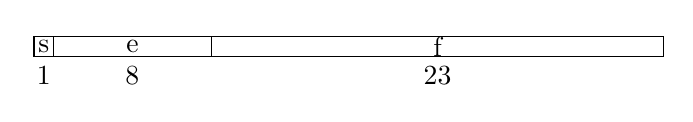
\begin{tikzpicture}
                    \draw (0, 0) rectangle (0.25, 0.25);
                    \node at (0.125, 0.125) {s};
                    \node at (0.125, -0.25) {1};

                    \draw (0.25, 0) rectangle (2.25, 0.25);
                    \node at (1.25, 0.125) {e};
                    \node at (1.25, -0.25) {8};

                    \draw (2.25, 0) rectangle (8, 0.25);
                    \node at (5.125, 0.125) {f};
                    \node at (5.125, -0.25) {23};
                \end{tikzpicture}
                \caption{IEEE 754 单精度浮点数示意图}
                \label{fig:NumberSystemBasics/FloatingPointNotations/IEEE754/BasicFormats/Single}
            \end{figure}

            并定义:
            \begin{enumerate}
                \item 如果 $e$ 是 $255$ 且 $f$ 不为 $0$(形如 $s\ 11111111\ bbbb \cdots bbbb$),那么其表示的值为 NaN;
                \item 如果 $e$ 是 $255$ 且 $f$ 为 $0$(形如 $s\ 11111111\ 0000 \cdots 0000$),那么其表示的值为 $(-1)^s\infty$(即正负无穷大);
                \item 如果 $e$ 在 $0$(不含)和 $255$(不含)之间(通常情况),那么其表示的值为 $(-1)^s2^{e-127}(1 \cdot f)$;
                \item 如果 $e$ 为 $0$ 但 $f$ 不为 $0$(形如 $s\ 00000000\ bbbb \cdots bbbb$),那么其表示的值为非规格化浮点数 $(-1)^s2^{-126}(0 \cdot f)$;
                \item 如果 $e$ 和 $f$ 均为 $0$(形如 $s\ 000000000\ 0000 \cdots 0000$),那么其表示的值为 $(-1)^s0$(即正负 $0$)。
            \end{enumerate}

            双精度浮点数由 $64$ 位二进制数组成,从左到右分别是 $1$ 位符号位 $s$,$11$ 位偏移指数 $e$ 和 $52$ 位分数 $f$,如图~\ref{fig:NumberSystemBasics/FloatingPointNotations/IEEE754/BasicFormats/Double} 所示,
            \begin{figure}
                \centering
                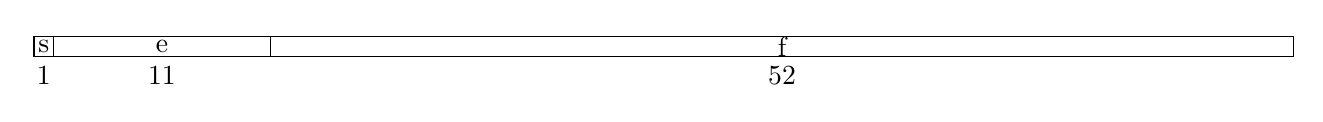
\begin{tikzpicture}
                    \draw (0, 0) rectangle (0.25, 0.25);
                    \node at (0.125, 0.125) {s};
                    \node at (0.125, -0.25) {1};

                    \draw (0.25, 0) rectangle (3, 0.25);
                    \node at (1.625, 0.125) {e};
                    \node at (1.625, -0.25) {11};

                    \draw (3, 0) rectangle (16, 0.25);
                    \node at (9.5, 0.125) {f};
                    \node at (9.5, -0.25) {52};
                \end{tikzpicture}
                \caption{IEEE 754 双精度浮点数示意图}
                \label{fig:NumberSystemBasics/FloatingPointNotations/IEEE754/BasicFormats/Double}
            \end{figure}

            并定义:
            \begin{enumerate}
                \item 如果 $e$ 是 $2047$ 且 $f$ 不为 $0$(形如 $s\ 11111111111\ bbbb \cdots bbbb$),那么其表示的值为 NaN;
                \item 如果 $e$ 是 $2047$ 且 $f$ 为 $0$(形如 $s\ 11111111111\ 0000 \cdots 0000$),那么其表示的值为 $(-1)^s\infty$(即正负无穷大);
                \item 如果 $e$ 在 $0$(不含)和 $2047$(不含)之间(通常情况),那么其表示的值为 $(-1)^s2^{e-1023}(1 \cdot f)$;
                \item 如果 $e$ 为 $0$ 但 $f$ 不为 $0$(形如 $s\ 00000000000\ bbbb \cdots bbbb$),那么其表示的值为非规格化浮点数 $(-1)^s2^{-1022}(0 \cdot f)$;
                \item 如果 $e$ 和 $f$ 均为 $0$(形如 $s\ 00000000000\ 0000 \cdots 0000$),那么其表示的值为 $(-1)^s0$(即正负 $0$)。
            \end{enumerate}

        \subsubsection{扩展格式}\label{subsubsec:NumberSystemBasics/FloatingPointNotations/IEEE754/ExtendedFormats}
            IEEE 754 还定义了单精度扩展格式和双精度扩展格式所需要遵守的规范,如表格~\ref{tab:NumberSystemBasics/FloatingPointNotations/IEEE754/ExtendedFormats/Requirements} 所示,但是对具体实现方式不做出任何要求。

            \begin{table}
                \centering
                \begin{tabular}{lrrrr}
                    参数       & 单精度 &        单精度扩展 &  双精度 &         双精度扩展 \\ \hline
                    $p$        &   $24$ &    $\geqslant 32$ &    $53$ &     $\geqslant 64$ \\
                    $E_{\max}$ & $+127$ & $\geqslant +1023$ & $+1023$ & $\geqslant +16383$ \\
                    $E_{\min}$ & $-126$ & $\leqslant -1022$ & $-1022$ & $\leqslant -16382$ \\
                    指数偏移量 & $+127$ &            未指定 & $+1023$ &             未指定 \\
                    指数位数   &    $8$ &    $\geqslant 11$ &    $11$ &     $\geqslant 15$ \\
                    总位数     &   $32$ &    $\geqslant 43$ &    $64$ &     $\geqslant 79$
                \end{tabular}
                \caption{IEEE 754 描述的四种浮点数格式的要求}
                \label{tab:NumberSystemBasics/FloatingPointNotations/IEEE754/ExtendedFormats/Requirements}
            \end{table}

        另外,IEEE 754 还定义了浮点数相关的运算等,由于本章仅关注记数基础,因此运算相关的会放到后面进行讲解。
